\documentclass{report}
\usepackage[spanish]{babel}
\usepackage{amsmath}



\usepackage[spanish]{babel}
\usepackage[utf8x]{inputenc}
\usepackage{amsmath}
\usepackage{graphicx}
\usepackage[colorinlistoftodos]{todonotes}
\usepackage{enumitem}
\usepackage{listings}
\usepackage{verbatim}
\usepackage{eurosym}
\usepackage[export]{adjustbox}
\usepackage{amssymb}
\usepackage{bussproofs}
\usepackage{amsmath}
\usepackage{tikz}
\usepackage{xcolor}
\usepackage{listings}
\usepackage{titletoc}
\usepackage{hyperref}

\hypersetup{
  colorlinks=true,
  linkcolor=black,
  urlcolor=blue,
  citecolor=black
}

\newcommand{\coverPage}[6]{%
%----------------------------------------------------------------------------------------
%	COVER START
%----------------------------------------------------------------------------------------
\begin{titlepage}

    \newcommand{\HRule}{\rule{\linewidth}{0.5mm}}
    \newcommand{\department}{#1}
    \newcommand{\course}{#2}
    \newcommand{\titleValue}{#3}
    \newcommand{\subtitleValue}{#4}
    \newcommand{\authorName}{#5}

    \center

    %----------------------------------------------------------------------------------------
    %	HEADER
    %----------------------------------------------------------------------------------------
    
\includegraphics{images/logo_usa.png}
    \vspace{0.5cm}
    \textsc{\Large \department}\\[0.5cm]
    \textsc{\Large \course}\\[0.5cm]
    \vfill

    %----------------------------------------------------------------------------------------
    %	TITLE
    %----------------------------------------------------------------------------------------

    \HRule\\
    \Huge
    \textbf{\titleValue}\\[0.5cm]
    \Large
    \textbf{\subtitleValue}\\
    \HRule\\[0.5cm]

    %----------------------------------------------------------------------------------------
    %	AUTHOR AND DATE
    %----------------------------------------------------------------------------------------

    \vfill
    \Large
    \textit{\authorName}\\
    {\large \today}\\[2cm]

\end{titlepage}
%----------------------------------------------------------------------------------------
%	COVER END
%----------------------------------------------------------------------------------------
}

\begin{document}
    \coverPage{ Matemáticas }{ Matemática Discreta }{ Tarea 3 }{  }{ Alexander Mendoza }{\today}

    \pagebreak
    \subsection*{Tarea 3}

1. En una caja hay 200 bombillas de las cuales 10 están averiadas. Si se seleccionan 15 bombillas al azar:

(a) ¿ Cuál es la probabilidad de que todas estén en buen estado?

Usando combinatorios:

$$P(\text{todas en buen estado}) = \frac{{\binom{190}{15}}}{{\binom{200}{15}}}$$

(b) ¿Cuál es la probabilidad de seleccionar no más de 4 bombillas averiadas?

$$P(\text{no más de 4 averiadas}) = \frac{{\binom{190}{15}}}{{\binom{200}{15}}} + \frac{{\binom{190}{14} \cdot \binom{10}{1}}}{{\binom{200}{15}}} + \frac{{\binom{190}{13} \cdot \binom{10}{2}}}{{\binom{200}{15}}} + \frac{{\binom{190}{12} \cdot \binom{10}{3}}}{{\binom{200}{15}}} + \frac{{\binom{190}{11} \cdot \binom{10}{4}}}{{\binom{200}{15}}}$$

2. Una baraja ordinaria tiene 52 cartas que están distribuidas en cuatro palos: treboles, corazones, picas y diamantes. Cada palo tiene 13 denominaciones.

(a) Si se realizan 4 extracciones sin reemplazo, ¿cuál es la probabilidad de sacar una carta de cada palo?

$$P(\text{Carta cada palo}) = P(\text{1ra extracción}) \cdot P(\text{2da extracción}) \cdot P(\text{3ra extracción}) \cdot P(\text{4ta extracción})$$

$$P(\text{Carta cada palo}) = 1 \cdot \frac{39}{51} \cdot \frac{26}{50} \cdot \frac{13}{49}$$

$$P(\text{Carta cada palo}) = \frac{1014}{4998} \approx 0.2029$$

(b) Si se realizan 4 extracciones con reemplazo, ¿cuál es la probabilidad de sacar cartas de exactamente dos palos?

Dos cartas de un palo y dos cartas de otro palo: 
$$ P(2 \cap 2) = \binom{4}{2} \left(\frac{1}{4}\right)^2 \left(\frac{1}{4}\right)^2 = 6 \times \frac{1}{16} \times \frac{1}{16} $$

Tres cartas de un palo y una carta de otro palo: 
$$ P(3\cap 1) = \binom{4}{1} \left(\frac{1}{4}\right)^3 \left(\frac{1}{4}\right)^1 = 4 \times \frac{1}{64} \times \frac{1}{4} $$

Total:
\begin{align*}
    P(\text{Total}) &= P(\text{2 y 2}) + P(\text{3 y 1}) \\
    &= 6 \times \frac{1}{16} \times \frac{1}{16} + 4 \times \frac{1}{64} \times \frac{1}{4} \\
    &= \frac{3}{64} + \frac{1}{64} \\
    &= \frac{4}{64} \\
    &= \frac{1}{16} \\
    &\approx 0.0625
\end{align*}
    

3. Una moneda es alterada, con el fin de que la probabilidad de obtener una cara sea de $2 / 3$. Si la moneda se lanza 7 veces y los lanzamientos son independientes el uno del otro, ¿Cuál es la probabilidad de obtener cuatro caras?

$$P(\text{Cara}) = \binom{7}{4} \left(\frac{2}{3}\right)^4 \left(\frac{1}{3}\right)^{7-4} = 0.02560$$

4. Las máquinas $\mathrm{A}, \mathrm{B}$ y $\mathrm{C}$ producen todas las mismas dos piezas $\mathrm{P} 1$ y P2. De todas las piezas producidas, la máquina A produce el $60 \%$, la B el $25 \%$ y la C el $15 \%$. Además, el $40 \%$ de las piezas hechas por A son P1, el $50 \%$ de las piezas hechas por B son $\mathrm{P} 1$ y el $60 \%$ de las piezas hechas por C son P1. En un muestreo aleatorio se obtuvo una pieza P1. Calcule las probabilidades de que la pieza provenga de la máquina A, B o C.

Usando regla de Bayes tenemos

$$P(A|P1) = \frac{0.40 \cdot 0.60}{0.40 \cdot 0.60 + 0.50 \cdot 0.25 + 0.60 \cdot 0.15}$$

5. La siguiente es la matriz de adyacencia de un grafo $G$ que representa un poligono industrial. Los vértices representan las torres de destilación y las aristas los caminos que las comunican. Etiquete los vértices desde $v_{1}$ hasta $v_{11}$ de izquierda a derecha y de arriba a abajo.

$$
\left(\begin{array}{lllllllllll}
0 & 1 & 1 & 0 & 0 & 0 & 0 & 0 & 0 & 0 & 0 \\
1 & 0 & 1 & 1 & 1 & 0 & 0 & 0 & 0 & 0 & 0 \\
1 & 1 & 0 & 1 & 0 & 1 & 0 & 0 & 0 & 0 & 0 \\
0 & 1 & 1 & 0 & 1 & 0 & 0 & 0 & 0 & 0 & 0 \\
0 & 1 & 0 & 1 & 0 & 0 & 0 & 0 & 0 & 1 & 0 \\
0 & 0 & 1 & 0 & 0 & 0 & 1 & 0 & 0 & 1 & 0 \\
0 & 0 & 0 & 0 & 0 & 1 & 0 & 0 & 1 & 1 & 0 \\
0 & 0 & 0 & 0 & 0 & 0 & 0 & 0 & 1 & 1 & 0 \\
0 & 0 & 0 & 0 & 0 & 0 & 1 & 1 & 0 & 1 & 1 \\
0 & 0 & 0 & 0 & 1 & 1 & 1 & 1 & 1 & 0 & 0 \\
0 & 0 & 0 & 0 & 0 & 0 & 0 & 0 & 1 & 0 & 0
\end{array}\right)
$$

(a) Dibuje el grafo correspondiente.

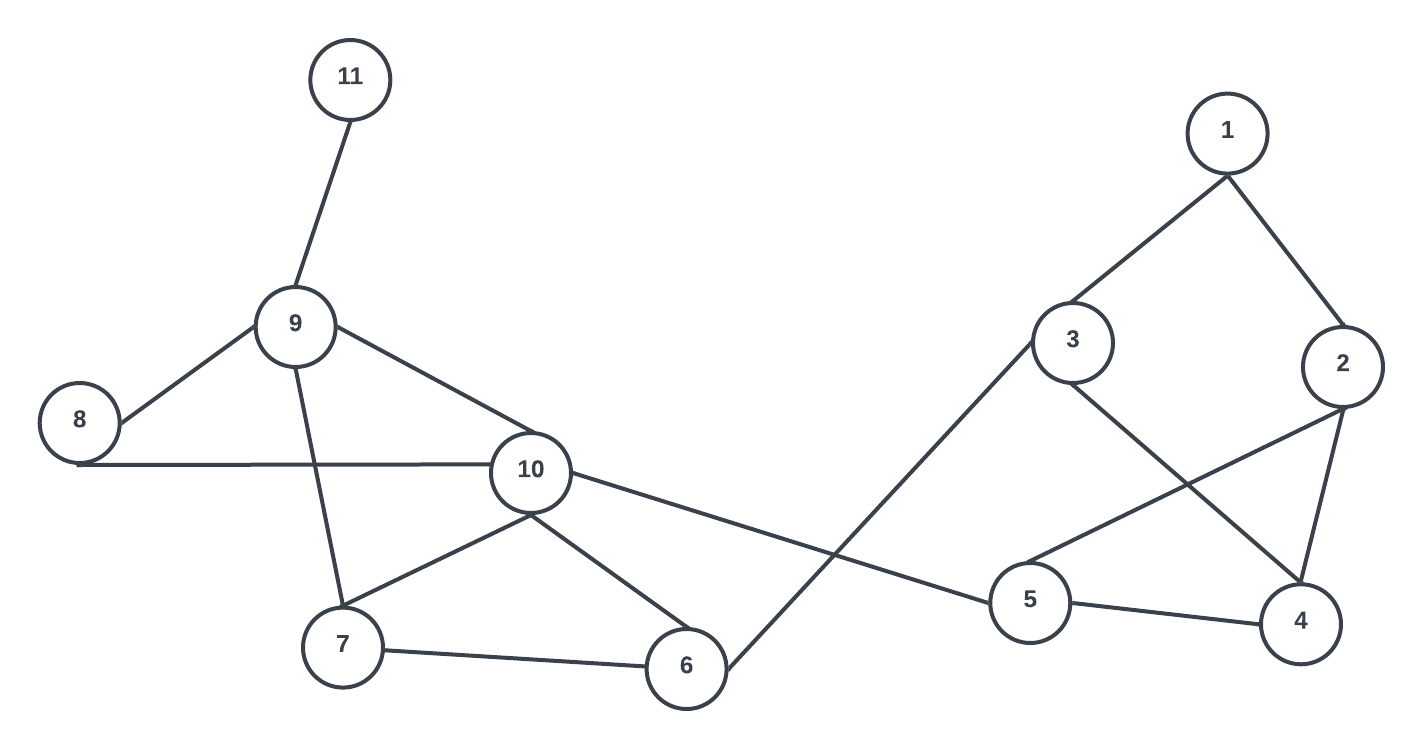
\includegraphics[width=1\textwidth]{images/graph1.png}

(b) Cada día se realiza la limpieza de los caminos del poligono empezando en la torre $v_{10}$ y terminando en la torre $v_{11}$. Use el algoritmo de Fleury para encontrar un sendero euleriano óptimo para la limpieza.

(c) Construya la matriz de incidencia del grafo.
\[
\left(\begin{array}{ccccccccccccccc}
1 & 1 & 0 & 0 & 0 & 0 & 0 & 0 & 0 & 0 & 0 & 0 & 0 & 0 & 0 \\
1 & 0 & 1 & 1 & 0 & 1 & 0 & 0 & 0 & 0 & 0 & 0 & 0 & 0 & 0 \\
0 & 1 & 1 & 0 & 1 & 0 & 0 & 1 & 0 & 0 & 0 & 0 & 0 & 0 & 0 \\
0 & 0 & 0 & 1 & 1 & 0 & 1 & 0 & 0 & 0 & 0 & 0 & 0 & 0 & 0 \\
0 & 0 & 0 & 0 & 0 & 1 & 1 & 0 & 0 & 0 & 0 & 1 & 0 & 0 & 0 \\
0 & 0 & 0 & 0 & 0 & 0 & 0 & 1 & 1 & 0 & 0 & 0 & 1 & 0 & 0 \\
0 & 0 & 0 & 0 & 0 & 0 & 0 & 0 & 1 & 1 & 0 & 0 & 0 & 1 & 0 \\
0 & 0 & 0 & 0 & 0 & 0 & 0 & 0 & 0 & 0 & 1 & 0 & 0 & 0 & 1 \\
0 & 0 & 0 & 0 & 0 & 0 & 0 & 0 & 0 & 1 & 1 & 0 & 0 & 0 & 0 \\
0 & 0 & 0 & 0 & 0 & 0 & 0 & 0 & 0 & 0 & 0 & 1 & 1 & 1 & 1 \\
0 & 0 & 0 & 0 & 0 & 0 & 0 & 0 & 0 & 0 & 0 & 0 & 0 & 0 & 0 \\
\end{array}\right)
\]
6. Una empresa a nivel nacional tiene oficinas en 9 ciudades. La empresa tiene un contrato con una compañía que proporciona líneas de teléfono entre las distintas oficinas. El costo anual en cientos de dólares de mantener una línea directa entre dos oficinas de acuerdo a la negociación con la compañía de teléfonos se muestra en el siguiente diagrama (Cada círculo representa una oficina)

Grafo:

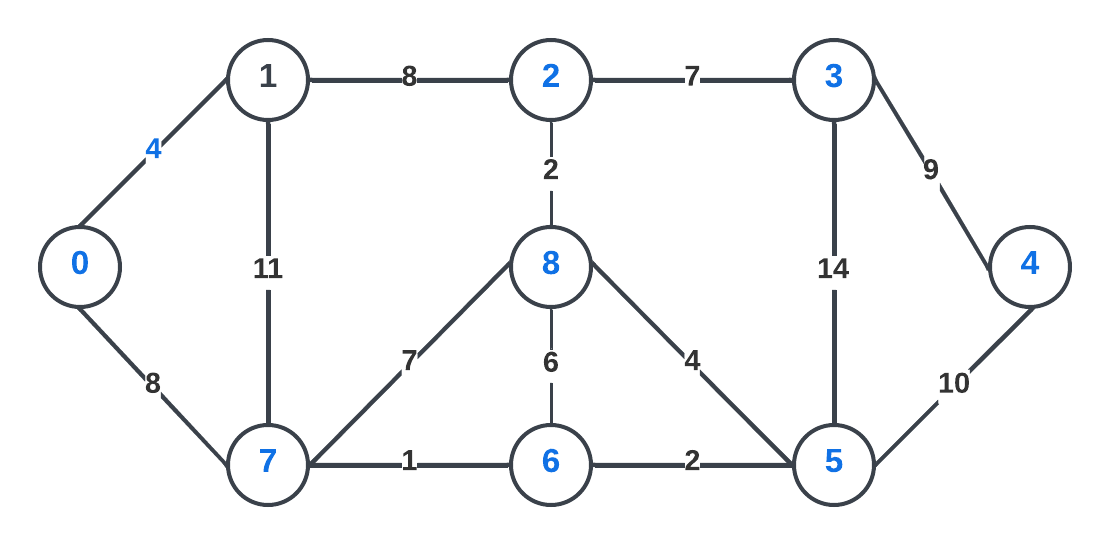
\includegraphics[width=1\textwidth]{images/graph2.png}

Grafo de menor costo:

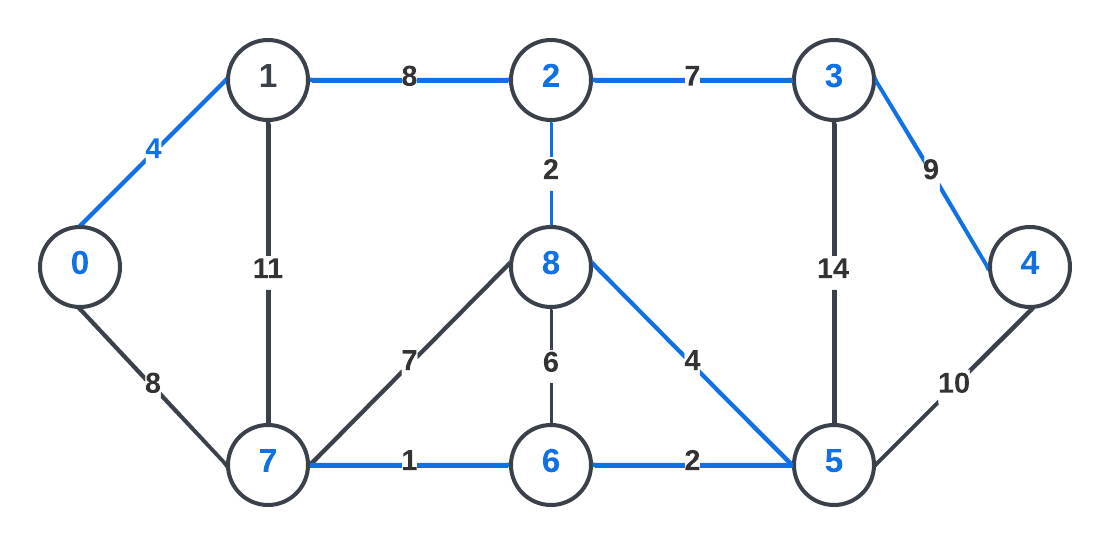
\includegraphics[width=1\textwidth]{images/graph3.png}


\end{document}
